<<<<<<< HEAD
%--------------------Preamble---------------------------------
\documentclass[journal]{IEEEtran}
\usepackage{blindtext}
\usepackage{graphicx}
\usepackage{amsmath}
\usepackage{pdfpages}
\usepackage{hyperref}
\usepackage{pdfpages}

\hypersetup{
	colorlinks = true,
	citecolor = {blue},
	urlcolor = {black}
}

\graphicspath{ {Pictures/} }

\markboth{North Dakota State University, December~2015}%
{Shell \MakeLowercase{\textit{et al.}}: Bare Demo of IEEEtran.cls for Journals}

\title{Using Dielectric Spectroscopy in Radio Frequencies to Measure Membrane Potential of Mouse Hypridoma cells}
\author{Andrew Bossert, Christopher Jordan - Denny, Nicolette Lippert}

\begin{document}

\maketitle

%----------------------Abstract---------------------------------

\begin{abstract}
This article explores using dielectric spectroscopy in an attempt to measure the trans-membrane potential of mouse hypridoma cells in the radio frequency spectrum. The purpose of this test is to "mimic" a capacitor with the cell suspension acting as a dielectric. This is a non-invasive way to measure the average membrane potential across your cell suspension and has been proven in \cite{Dielectric Spectroscopy} for frequencies up to \textbf{$10^5 Hz$}.
\end{abstract}

\section{Implications of Membrane Potential}
Although there may be many implications of transmembrane potential at radio frequencies, the focus of this example is in disease models. In the late 1930's it was suggested that a relationship lie between cancer and the bioelectric properties of host tissue. Interestingly, membrane voltage ($V_{mem}$) analysis in many different mammalian cell types reveals that proliferative (to grow by rapid production of new parts) potential is correlated with unique ranges of $V_{mem}$ : quiescent cells (cells withdrawn from the cell cycle and do not proliferate) tend to be hyperpolarized (more negative), whereas highly plastic cells such as embryonic cells, adult stem cells and tumors cells are depolarized (more positive). \cite{TMP-implications}. During the early stages of tumor formation, $V_{mem}$ is a key regulator of the cell cycle and determines the proliferative state of many different kinds of cells. These statements excite the possibility of non-invasive techniques being used to track bioelectric cell states and detection of tumors, or even mitigation of tumor formation by canonical oncogene (gene that has potential to cause cancer).

\section{Hypothesis}
Mouse hybridoma cells when exposed to a range of radio frequencies will have a constant relative dielectric permittivity, when using dielectric spectroscopy. 

\section{Calculating Membrane Potential}
Modeling the impedance of the cell suspension as a resitor $R = d/\sigma A$ in parallel with a capacitor $C = \epsilon A/d$, where $\sigma$ and $\epsilon$ are the conductivity and dielectric permittivity of the cell suspension, and $A$ and $d$ are the surface area of the two disk electrodes and the distance between them. 

\begin{equation}
\label{conductivity}
\sigma(\omega) = \frac{d}{AZ}
\end{equation}

\begin{align*}
C &= \frac{1}{sZ},s=j\omega \\
\frac{1}{sZ} &= \frac{\epsilon_r \epsilon_0 A}{d} \\
\epsilon_r &= \frac{d}{s\epsilon_0 AZ}
\end{align*}

\begin{equation}
\label{permittivity}
\epsilon_r(\omega) = Im\frac{d}{\epsilon_0\omega AZ}
\end{equation}

\begin{equation}
\mathcal Z^S-Z^P = Z^O \\
\end{equation}

$Z^S$ is the sample impedance, $Z^P$ is the unknown device impedance, and $Z^O$ is the measured impedance. \\

\section{Distance Between Plates:}
The near and far field transmission will depend on plate distance. The most agreed upon definition of near field transmission is less than one wavelength($\lambda$) away \cite{near-far-em}. Considering a sinusoidal wave traveling at a constant speed, the wavelength can be calculated with the following formula \ldots

\begin{equation}
\label{wavelength}
\lambda = \frac{v}{f}
\end{equation}

$v$ is the magnitude of the phase velocity and $f$ is the frequency of the sinusoid. It is difficult to determine the phase velocity of our electromagnetic wave while propagating through the cell suspension, but considering water, a prediction of the wavelength can be made. The velocity of EM waves is more than 4 orders faster than acoustic waves according to \cite{wave-propagation-water}. Knowing that the speed of sound is $343.2 m/s$ we can say \ldots

\begin{equation}
\label{near-wavelength-water}
\lambda = \frac{343.2 \cdot 4}{10^9} = 1.3728 \times 10^{-6} m
\end{equation}

Water is a good basis for the phase velocity as the cell suspension is made from distilled $H_2O$ and mouse hybridoma cells. $10^9 Hz$ will be used as the minimum radio frequency. The micrometer is sensitive to $10\mu m$, thus the test fixture will be capable of measuring only waves 10 times greater than the fundamental wavelength; meaning far field transmissions will be measured. This is a satisfactory result, as the far field is the "real" radio waves that propagate through space at relatively the speed of light \cite{near-far-em}. 

\section{S-Parameters}
At low frequencies it is common to use the transfer and impedance matrices, since this experiment uses high frequencies, scattering parameters are more preferable. A linear two-port network is used to characterize the equivalent circuit parameters for our experiment. More specifically, scattering parameters are used to relate the outgoing waves $b_1,b_2$ to the incoming waves $a_1,a_2$. The parameters $S_{11},S_{22}$ are the reflection coefficients, or the ratio of the amplitude of the reflected wave to the incident wave. The parameters $S_{21},S_{12}$ are the transmission coefficients, or the amplitude, intensity or total power of a transmitted wave relative to a incident wave (power of propagation through a medium). As a reminder, the incident wave is the wave traveling from source to load, as the reflected wave is the traveling from load to source.

\begin{figure}[ht]
\label{Equivalent_Circuit}
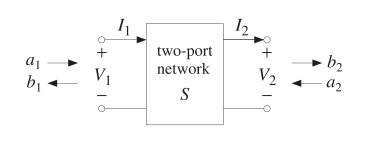
\includegraphics[width=8cm]{two_port.png}
\end{figure}

\begin{figure}[ht]
\label{Equivalent_Circuit}
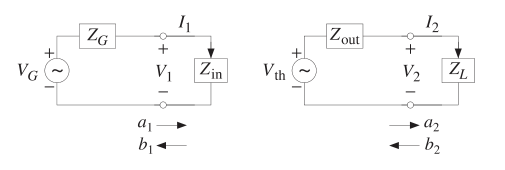
\includegraphics[width=8cm]{Equivalent_Circuit.png}
\end{figure}

\begin{align*}
\label{s-conversion-z}
Z_{11} &= Z_0\frac{(1+S_{11})(1-S_{22})+S_{12}S_{21}}{ (1-S_{11})(1-S_{22})-S_{12}S_{21}} \\
Z_{12} &= Z_0\frac{2S_{12}}{ (1-S_{11})(1-S_{22})-S_{12}S_{21}} \\
Z_{21} &= Z_0\frac{2S_{21}}{ (1-S_{11})(1-S_{22})-S_{12}S_{21}} \\
Z_{22} &= Z_0\frac{ (1-S_{11})(1+S_{22})+S_{12}S_{21}}{ (1-S_{11})(1-S_{22})-S_{12}S_{21}}
\end{align*}

The found S-Parameters can be converted to Z-parameters to get the model of the Device Under Test (DUT) as shown in the resistor network above.

\section{Transmembrane Potential}
It is generally accepted that the cell membrane can be represented by a dielectric shell$(\epsilon_1,\sigma_1)$. The core can be described by $(\epsilon_2,\sigma_2)$. These live cells contain negative charges inside and attract the positive charges, mainly potassium and soidium ions on the outside. The dielectric response of live cells is fundamentally different than dead cells. The main difference between the two is the membrane potential in live cells. The effect of the membrane potential is an accumulation of mobile electric charge carriers at the membrane surfaces. When introducing a time-oscillating electric field, these charges move on the surface of the membrane. Since the mobility of these surface charges is relatively small, this effect appears only at low frequencies, typically $<10kHz$. In this range the relative dieletric permittivity of live cell suspensions can be as high as $10^6$. This phenomenon is know as the $\alpha-$relaxation effect\cite{dielectric-response}. There is a sharp frequency above which the ions can no longer follow the electric field. Above this frequency, the polarizability of the cells drastically decreases and the $\alpha$-effect disappears.

\section{Materials}

\begin{figure}[h]
\label{test-fixture}
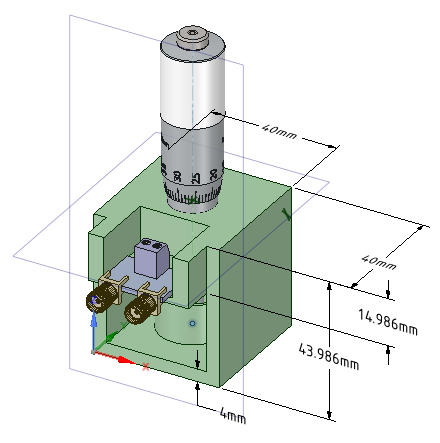
\includegraphics[width=8cm]{Combined_Test_Fixture.png}
\end{figure}

\subsection{Copper Plates}
Two copper plates $3/4 \: inch$ in diameter will be used. One plate will be fixed to the bottom of the beaker and the other is attached to a micrometer. To create the copper plates a hole puncher will be used.

\subsection{Copper Wire Leads}
Two wires will be attached to the copper plates. The wire attached to the fixed bottom plate will be attached to the center, and run through the bottom of the test fixture to later be attached to a network analyzer. The second wire will be attached to top plate on one of the edges and run up the side of the beaker to be attached to a network analyzer. These two wires will provide the radio frequency signal and the probes to be attached to a network analyzer.

\subsection{3-D printed Beaker}
A 3-D printed beaker will be made to perfectly fit the test fixture. The beaker will be made of ABS plastic and is used to hold the cell suspension and two copper plates. It will be placed in the center of the test fixture stand.

\subsection{Micrometer}
A micrometer will be used to adjust the height of one of the copper plates. The micrometer will be attached to the test fixture stand, and the drive of the micrometer will be attached to one of the copper plates. A micrometer cap will be 3-D printed in ABS plastic to perfectly fit the micrometer and later be adhered to the copper plate.

\subsection{Test Fixture Stand}
The test fixture stand will provide a base for the beaker as well as an accurate and stable micrometer mount.This item will be 3D printed with ABS plastic.

\subsection{Cells}
Cells will consist of a line of SP 2/0 myelomas hypridoma. These are nonadherent cells, and are cancer cells from mice.\cite{mouse-myeloma-hybridoma-strain} They are rated at biosafety level 1. This level is suitable for work involving well-characterized agents not known to consistently cause disease in healthy adult humans, and of minimal potential hazard to laboratory personnel and the environment. Research with these agents may be performed on standard open laboratory benches without the use of special containment equipment, and it is not necessary for Biosafety level 1 labs to be isolated from the general building.\cite{biosafety-levels}

\subsection{Hewlett-Packard 8735E Network Analyzer 30kHz - 6GHz}
Used with this network analyzer was the Agilent 11857D 7mm test port returns($50\Omega$). This network analyzer will be used to gather our scattering parameters. This version features the 006 option which give it a 6 GHz upper frequency range.\\
Resolution: $1 Hz$ \\
Stability: typically $\pm7.5 ppm$ \\
Accuracy: $\pm10 ppm$\\
Resolution: $0.05 dB$

\begin{figure}[h]
\label{test-fixture}
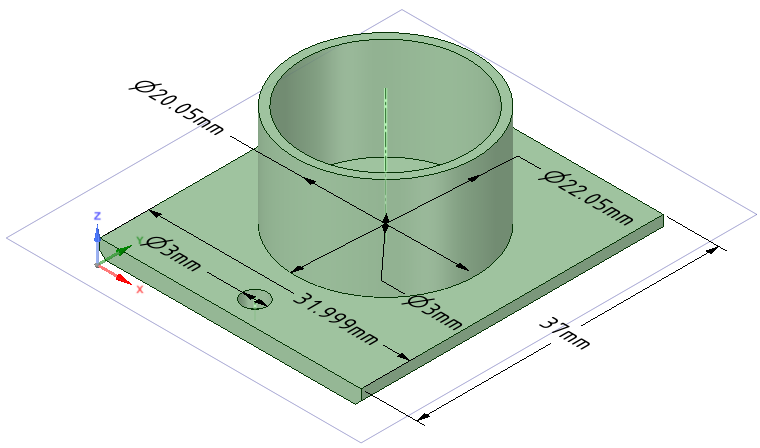
\includegraphics[width=8cm]{Beaker.png}
\end{figure}

\section{Methods}

\subsection{Procedure for splitting cells for regrowth and testing}
\subsection{Tools and Equipment}
\begin{itemize}
\item New cell culture flask
\item Centrifuge
\item 1ml centrifuge vials 
\item Pipette with 10ml graduated tips
\item Bleach
\item Phosphate buffer solution (PBS)
\item Cell food (10\% FBS PFS solution)
\item Vial rack for the centrifuge vials
\item 50ml sealable test tube
\end{itemize}

\subsection{Personal Safety Equipment}
For bio safety level 1, the use of gloves and a lab coat is required for personal protection. The cells are not to leave the bio safety level 1 lab room. This is a requirement set forth by those in charge of the biology lab.

\subsection{Notes}
\begin{itemize}
\item The cell suspension will become more acidic over time, yellow indicates optimal cell growth and orange indicates high acidity. Dark pink is the original color of PBS solution.
\item The cells are being kept under conditions of 37 $C\circ$ and 4.9\% CO2 in the incubation chamber when not in use. 
\end{itemize}

\subsection{Procedure}

\textbf{Centrifuging:}
\begin{enumerate}
\item Remove the flask from the incubator.
\item Using the pipettes, put 1 ml of cell solution from the cell culture flask into each of the centrifuge vials.
\item Seal the vials and evenly distribute them in a centrifuge. Dispose of any vials that would cause an odd number. Run the centrifuge at 1.7krpm for 5 min. Once complete, there will be a pellet of cells in the bottom of the vials.
\item Split the vials into two equal groups, one group will be used to create the solution for testing and the other will be used for regrowth.
\end{enumerate}

\textbf{For cell regrowth:}
\begin{enumerate}
\item Siphon off the solution in the vials and put it in the test tube. 
\item Using a new pipette, add 1ml of food to the vials. Note, the tip of the pipette should not touch the cells.
\item Shake the vials to dissolve the pellet.
\item Using a pipette, add the solution of cells and cell food to a new flask. The flask should be labeled with the type of cells or strain, and what path number they are on.
\item The flask is then sealed, and placed horizontally back in the incubation chamber until this process needs to be repeated.
\end{enumerate}

\textbf{Preparing Cells for testing:}
\begin{enumerate}
\item Repeat step 1 from the Cell regrowth section.
\item Using the pipette, add 1 ml of a buffer solution.
\item Repeat step 3 of the Cell Regrowth section.
\item Using the pipette, the solution can be added as needed to the test fixture. It can also be stored temporarily in test tube or a cell culture flask.
\end{enumerate}

\textbf{For unused centrifuge vials:}
\begin{enumerate}
\item Repeat step 1 from the Cell regrowth section.
\item Using the pipette, add 1ml of bleach to the vials.
\item Shake the vials to dissolve.
\item Using a pipette, the bleach and cell solution is added to the mixture of old cells in the disposable test tube. 
\end{enumerate}

\textbf{Clean up:} \\
Add several milliliters of bleach to the disposable test tube. The liquid should turn color from light blue to clear and can now be safely disposed. All surfaces and materials that are not disposable should be wiped down with 70\% ether solution. All disposable equipment can be discard in the bio-safe bins located near the hood. 

\section{Experiment Procedure (Network Analyzer)}

\textbf{Initial Setup}
\begin{itemize}
	\item Set a 10 mm spacing between the copper plates. The first plate is located where the micrometer reads 1 mm.
	\item Connect the Agilent 11857D 7mm test port returns($50\Omega$) between the network analyzer and the SMA connectors located on the test fixture. Both wires from the test fixture must be screwed into the lead terminals.
	\item Before moving the top plate to the desired position, insert 3.15ml of the fluid under test.
	\item Record all measurements to the floppy disc to be further processed.
\end{itemize}

\textbf{Measurements of S-Parameters:}
\begin{enumerate}
	\item Measure the S-Parameters of our device with air as a dielectric.
	\item Measure the S-Parameters with PBS (Phosphate Buffered Saline).
	\item Measure the S-Parameters with PBS Mouse Hybridoma solution.
\end{enumerate}

\section{Experimental Procedure (Impedance Analyzer)}

\textbf{Initial Setup}
\begin{itemize}
	\item Set the test beaker to 3 mm spacing between the copper plates. The first plate is located where the micrometer reads 1 mm. (a total of 2mm distance between plates)
	\item Connect the impedance analyzer leads to wires of test fixture.
	\item Before moving the top plate to the desired position, insert 0.57ml of the fluid under test.
	\item Record all measurements on the computer.
\end{itemize}

\textbf{Measurements of Impedance:}
\begin{enumerate}
	\item Measure the impedance of our device with air as a dielectric.
	\item Measure the impedance with PBS (Phosphate Buffered Saline).
	\item Measure the impedance with PBS Mouse Hybridoma solution.
\end{enumerate}

\textbf{Count Cell concentration} \\
The cell concentration will be measured using a hemocytometer. An example of the process of counting the cells can be seen in the next figure.

\begin{figure}[h]
\label{hemocytometer}
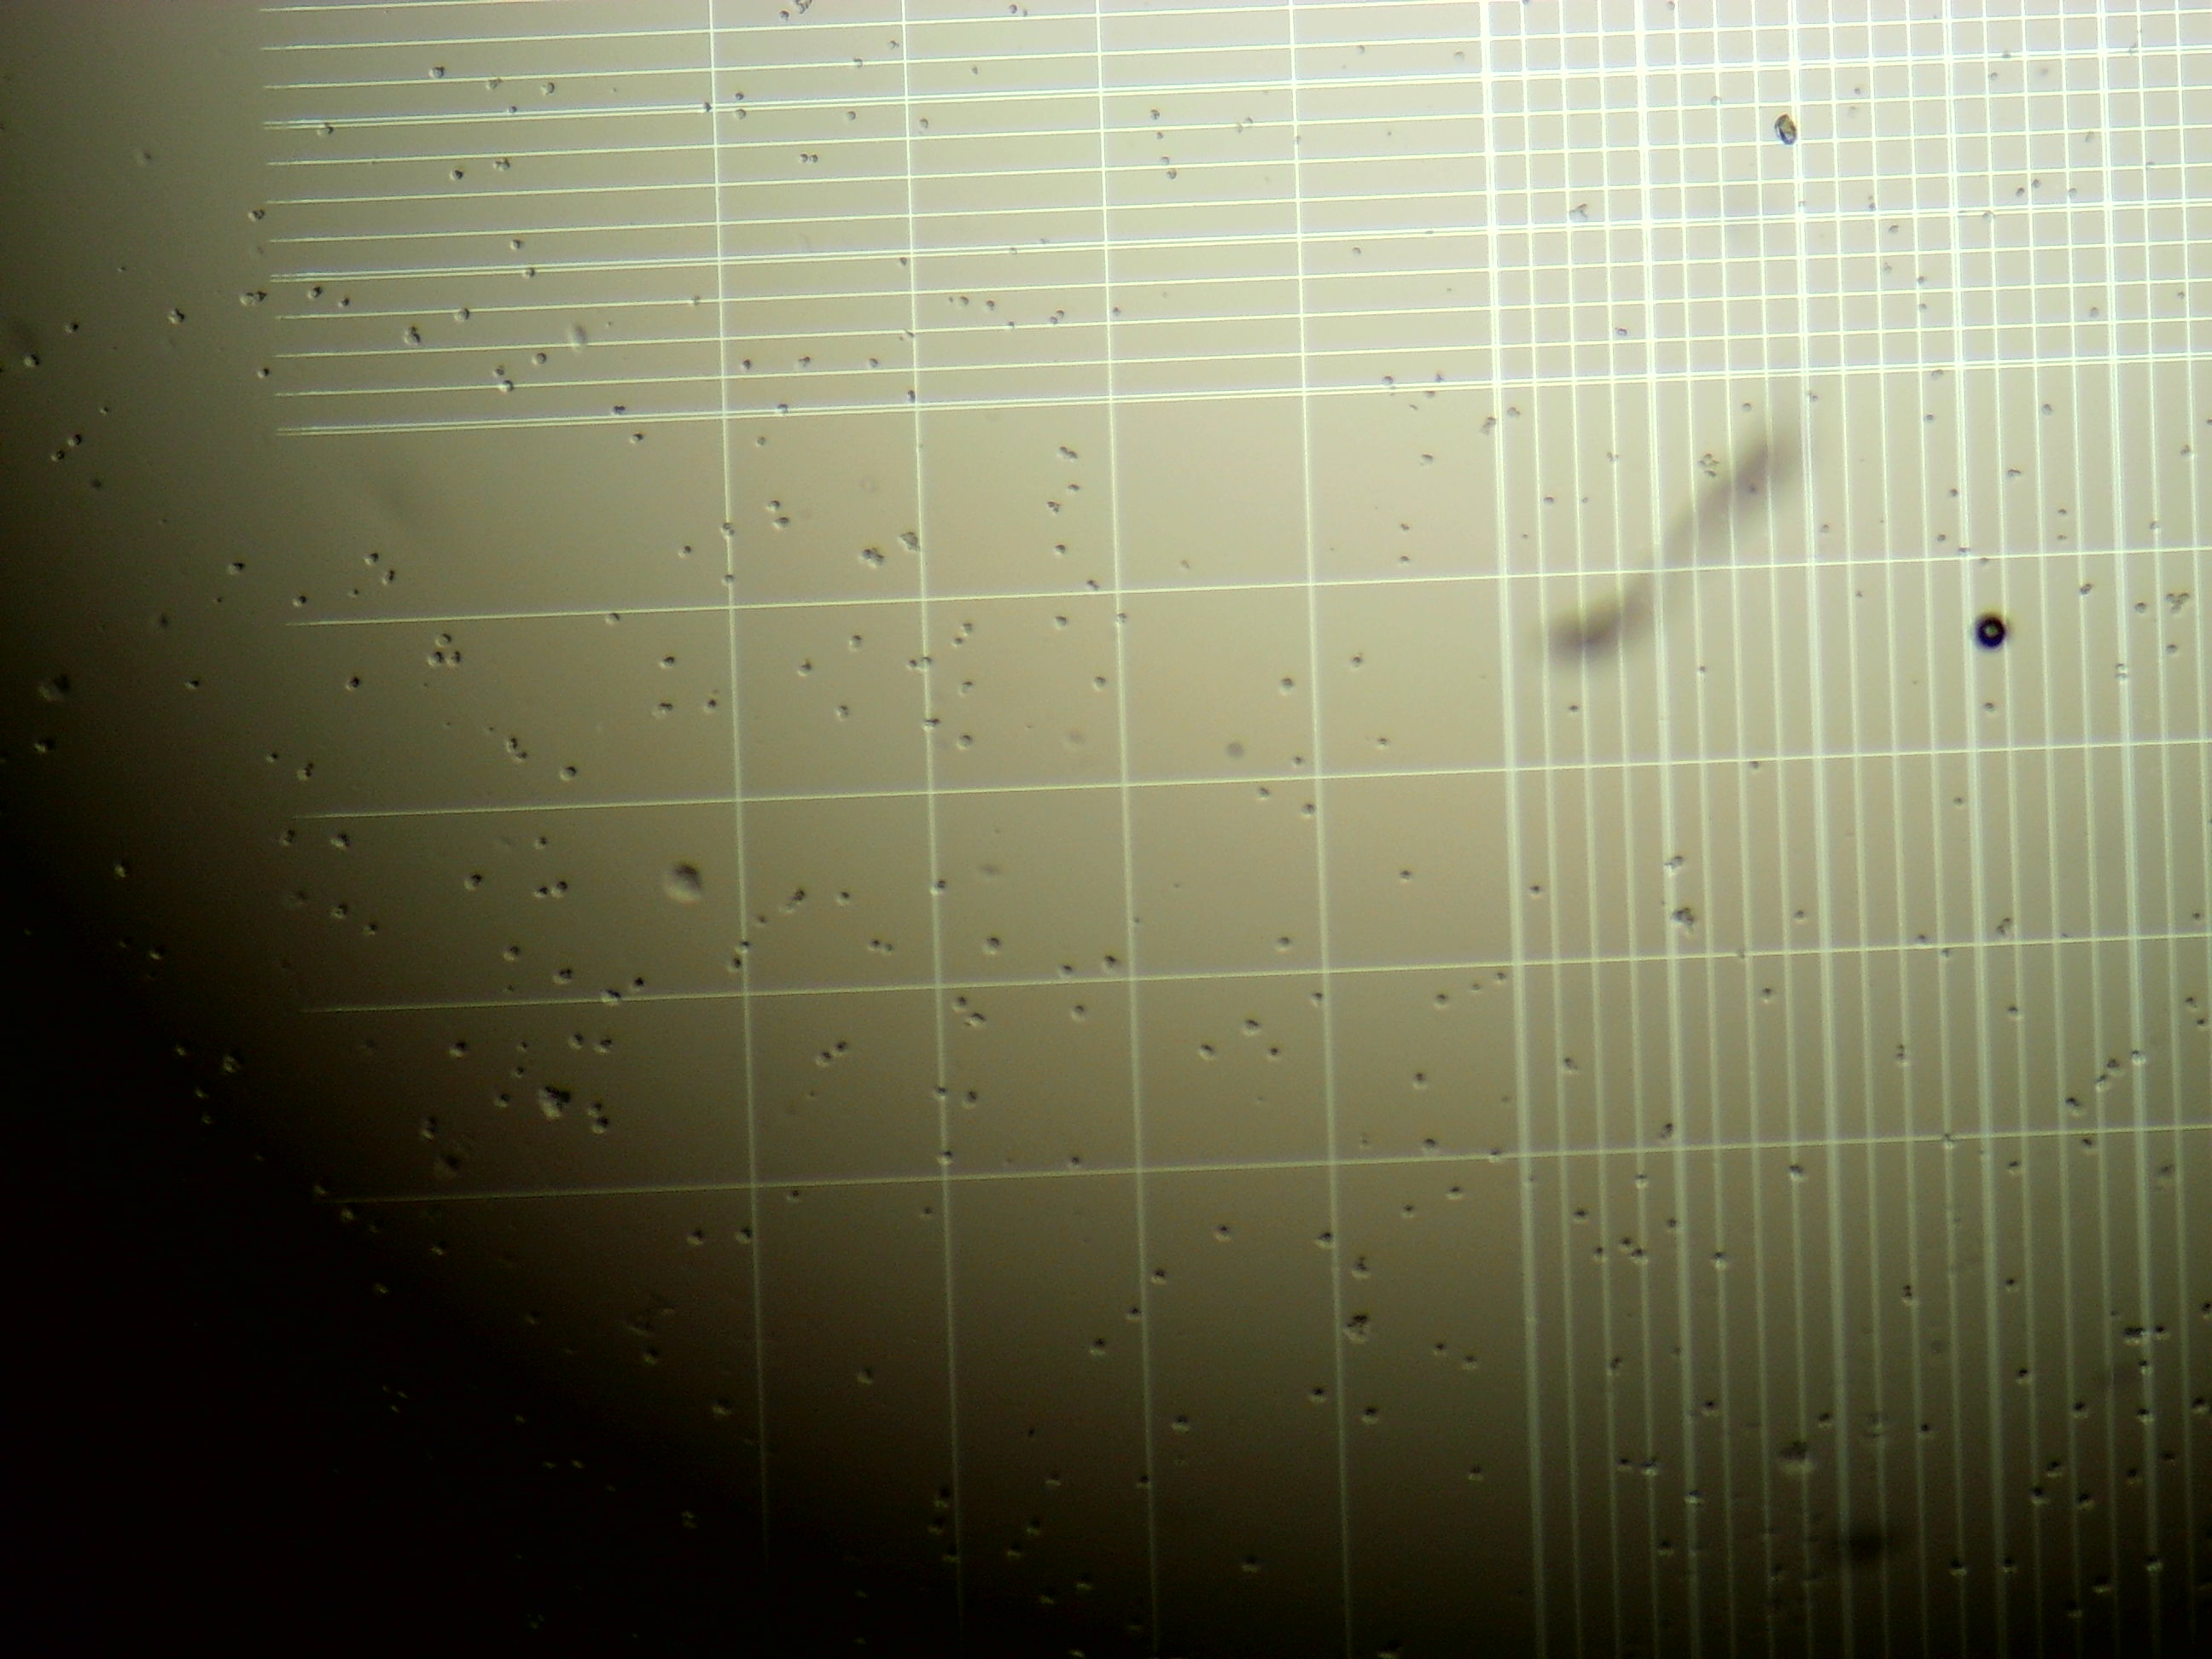
\includegraphics[width=9cm]{hemocytometer.jpg}
\end{figure}

\section{Data and Analysis}
The first three plots show the relative dielectric permittivity of the device under test. The device has been modeled by a resistor network and each of the permittivities have been calculated in the following figures using equation \ref{permittivity}.

\begin{align*}
Z_{in} &= Z_{11} - Z_{12} \\
Z_{p} &= Z_{12} \\
Z_{out} &= Z_{22} - Z_{12} \\
\end{align*} 

\begin{figure}[ht]
\label{diectric_Permittivity_in}
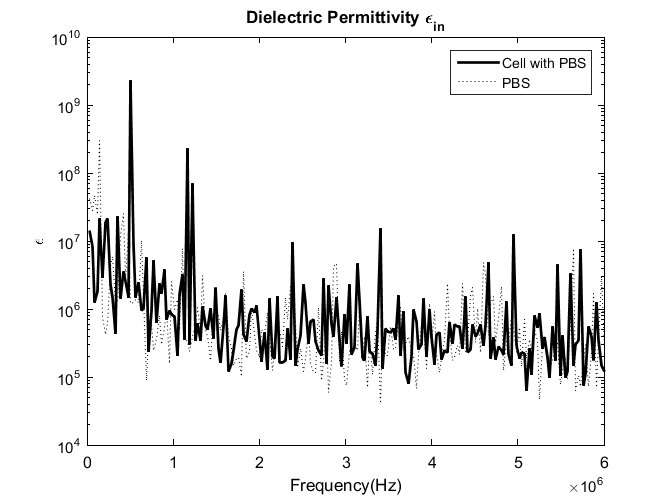
\includegraphics[width = 9cm]{Epsilon_In.png}
\end{figure}

\begin{figure}[ht]
\label{diectric_Permittivity_P}
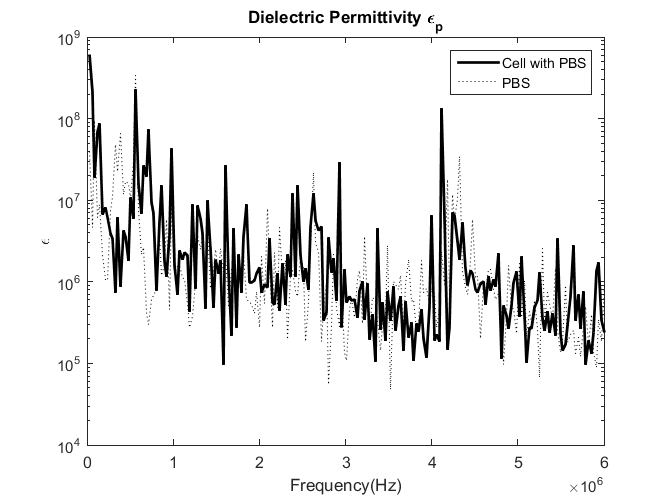
\includegraphics[width = 9cm]{Epsilon_P.png}
\end{figure}

\begin{figure}[ht]
\label{diectric_Permittivity_Out}
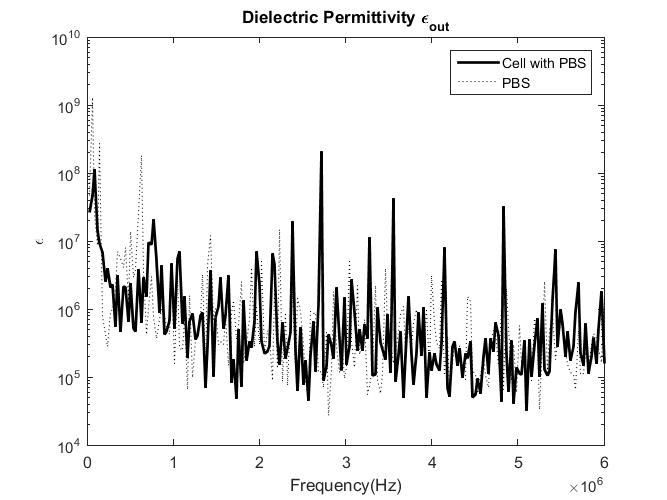
\includegraphics[width = 9cm]{Epsilon_Out.png}
\end{figure}

As illusrated in the graphs below, the relative permittivity of the cells in all cases is similar to the relative permittivity of the PBS solution. This implies that only the permittivity of the PBS solution and test fixture is measured. The relative permittivity is noticeably high, where the mean of the three relative permittivities is $7.5538\times10^6$. To put this in perspective, air has a relative permittivity of 1.0006. When looking at the results from experiment two at low frequencies, we see how the cells suspended in the PBS solution have a high permittivity and drops down with frequency. This is a trend that has been seen in research before such as in reference \cite{Dielectric Spectroscopy}. This area is known as the $\alpha$-relaxation region. At high frequencies, noise is also noticeable. 

\begin{figure}[ht]
\label{diectric_Permittivity_Low_Freq}
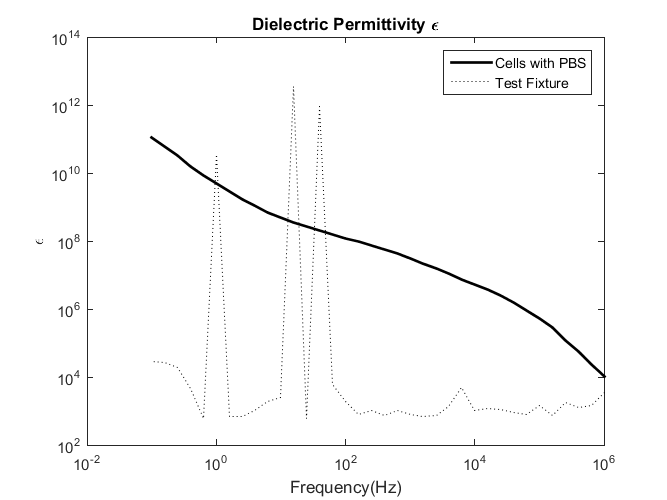
\includegraphics[width = 9cm]{Epsilon_Low_Freq.png}
\end{figure}

\section{Conclusion}
The hypothesis stated: when using dielectric spectroscopy, mouse hybridoma cells exposed to a range of radio frequencies would cause a constant relative dielectric permittivity. Having this constant relative permittivity would lead to the conclusion that no potential exists at radio frequencies, or that dielectric spectrosopy is not a viable solution to measure the trans-membrane potential at radio frequncies. A reason this may not be a viable solution is the radio-frequencies are passing through our dielectric as a short. When observing the impedance for a capacitor $Z = \frac{1}{j2\pi f C}$ notice that as the frequency increases the impedance lowers. This lower impedance is problematic when trying to use dielectric spectroscopy for measuring trans-membrane potential. It is also known from prior research that an $\alpha$-relaxation effect occurs at frequencies lower than 10 kHz. Above this frequency the ions can no longer follow the electric field, and the ions in the cell no longer have time to react to the electric field. Regarding the noise, it can be suppressed in a faraday cage. 

\section{Alternative Methods}
A report in 2001 was written on developing coplanar waveguide devices which can perform dielectric spectroscopy on biological samples within a microfluidic channel. Thses devices yield permittivity spectra across an exceptionally broad range of frequencies from 40 Hz to 26.5 GHz. At low frequencies, the polarization is able to closely follow the applied electric field ($\epsilon = \epsilon_{LF}$), while at high frequencies applied excitations oscillate too fast for the chrages to respond ($\epsilon=\epsilon_{HF}$), where generally $\epsilon_{LF} \gg \epsilon_{HF}$. By combining transmisstion line design with robust thin-film insulation, sensitivity to sample properties can be achieved in both low and high frequency regimes within a single device.

\section{Acknowledgement}
The authors would like to acknowledge Daniel Ewert and Jared Hansen for their leadership in this project. A special thanks to Dhamakeerthi Nawarathna for his help in the biology lab, and Matthew Kerns for editing this document.

\begin{thebibliography}{9}

\bibitem{Dielectric Spectroscopy}
C.Prodan \textit{et al.},
"Low-frequency, low-field dielectric spectroscopy of living cell suspensions,"
\textit{Journal of Applied Physics}, 2004.

\bibitem{wave-propagation-water}
Shan Jiang and Stavros Georgakopoulos,
"Electromagnetic Wave Propagation into Fresh Water,"
\textit{Journal of Electromagnetic Analysis and Applications},2011,pp.261-266.

\bibitem{near-far-em}
Lou Frenzel,
What is the Difference Between EM Near Field and Far Field
\textit{Electronic Design}, 2012.

\bibitem{TMP-implications}
Brook T.Chernet and Michael Levin,
Transmembrane voltage potential is an essential cellular parameter for the detection and control of tumor development in a Xenopus mode,l\textit{Disease Models \& Mechanisms}2013,pp.595-607.

\bibitem{biosafety-levels}
Center for Disease Control and Prevention
\textit{Recognizing the Biosafety Levels}.
\url{www.cdc.gov/training/QuickLearns/biosafety/}

\bibitem{mouse-myeloma-hybridoma-strain}
ATCC
\textit{Mouse Hybridoma (Sp 2/0), IMM010.51.2 (PTA-2360)}.
American Type Culture Collection

\bibitem{Electromagnetic Waves and Antennas}
Sophocles J. Orfanidis,
Electromagnetic Waves and Antennas
\textit{Rutgers University},1999

\bibitem{dielectric-response}
Emil Prodan \textit{et al.},
"The Dielectric Response of Spherical Live Cells in Suspension: An Analytic Solution," \textit{Biophysical Journal}, 2008

\bibitem{dielectric-spectroscopy-bioanalysis}
G.R. Facer \textit{et al.},
"Dielectric spectroscopy for bioanalysis: From 40 Hz to 26.5 GHz in a microfabricated wave guide," \textit{Applied Physics Letters}, 2001

\end{thebibliography}

\end{document}
=======
%--------------------Preamble---------------------------------
\documentclass[journal]{IEEEtran}
\usepackage{blindtext}
\usepackage{graphicx}
\usepackage{amsmath}
\usepackage{pdfpages}
\usepackage{hyperref}

\hypersetup{
	colorlinks = true,
	citecolor = {blue},
	urlcolor = {black}
}

\graphicspath{ {Pictures/} }

\markboth{North Dakota State University, December~2015}%
{Shell \MakeLowercase{\textit{et al.}}: Bare Demo of IEEEtran.cls for Journals}

\title{Measuring Transmembrane Potential of Mouse Hypridoma cell culture in Radio Frequency Spectrum}
\author{Andrew Bossert, Christopher Jordan - Denny, Nicolette Lippert}

\begin{document}

\maketitle

%----------------------Abstract---------------------------------

\begin{abstract}
This article explores using dielectric spectroscopy in an attempt to measure the trans-membrane potential of mouse hypridoma cells in the radio frequency spectrum. The purpose of this test is to "mimic" a capacitor with the cell suspension acting as a dielectric. This is a non-invasive way to measure the average membrane potential across your cell suspension and has been proven in \cite{Dielectric Spectroscopy} for frequencies up to \textbf{$10^5 Hz$}.
\end{abstract}

\section{Implications of Membrane Potential}
Although there may be many implications of transmembrane potential at radio frequencies, the focus of this example is in disease models. In the late 1930's it was suggested that a relationship lie between cancer and the bioelectric properties of host tissue. Interestingly, membrane voltage ($V_{mem}$) analysis in many different mammalian cell types reveals that proliferative (to grow by rapid production of new parts) potential is correlated with unique ranges of $V_{mem}$ : quiescent cells (cells withdrawn from the cell cycle and do not proliferate) tend to be hyperpolarized (more negative), whereas highly plastic cells such as embryonic cells,adult stem cells and tumors cells are depolarized (more positive). \cite{TMP-implications}. During the early stages of tumor formation, $V_{mem}$ is a key regulator of the cell cycle and determines the proliferative state of many different kinds of cells. These statements excite the possibility of non-invasive techniques being used to track bioelectric cell states and detection of tumors, or even mitigation of tumor formation by canonical oncogene (gene that has potential to cause cancer).

\section{Hypothesis}
When using dielectric spectroscopy, the mouse hybridoma cells when exposed to a range of radio frequencies will have a constant relative dielectric permittivity. 

\section{Calculating Membrane Potential}
We model the impedance of the cell suspension as a resitor $R = d/\sigma A$ in parallel with a capacitor $C = \epsilon A/d$, where $\sigma$ and $\epsilon$ are the conductivity and dielectric permittivity of the cell suspension and $A$ and $d$ are the surface area of the two disk electrodes and the distance between them. 

\begin{equation}
\label{conductivity}
\sigma(\omega) = \frac{d}{AZ}
\end{equation}

\begin{align*}
C &= \frac{1}{sZ},s=j\omega \\
\frac{1}{sZ} &= \frac{\epsilon A}{d} \\
\epsilon &= \frac{d}{sAZ}
\end{align*}

\begin{equation}
\label{permittivity}
\epsilon(\omega) = \frac{d}{\omega AZ}
\end{equation}

\begin{equation}
\mathcal Z^S-Z^P = Z^O \\
\end{equation}

Where $Z^S$ is the sample impedance, $Z^P$ is the unknown device impedance, and $Z^O$ is the measured impedance. \\

\section{Distance Between Plates:}
With regards to near and far field transmission. The most agreed upon definition of near field transmission is less than one wavelength($\lambda$) away \cite{near-far-em}. If we consider a sinusoidal wave traveling at a constant speed, we can calculate wavelength with the following formula \ldots

\begin{equation}
\label{wavelength}
\lambda = \frac{v}{f}
\end{equation}

Where $v$ is the magnitude of the phase velocity and $f$ is the frequency of the sinusoid. It is difficult to determine the phase velocity of our electromagnetic wave while propagating through our cell suspension, but if we consider water, we can make a prediction of the wavelength. The velocity of EM waves is more than 4 orders faster than acoustic waves according to \cite{wave-propagation-water}. Knowing that the speed of sound is $343.2 m/s$ we can say \ldots

\begin{equation}
\label{near-wavelength-water}
\lambda = \frac{343.2 \cdot 4}{10^9} = 1.3728 \times 10^{-6} m
\end{equation}

Water is a good basis for the phase velocity as the cell suspension is made from distilled $H_2O$ and mouse hybridoma cells. I used $10^9 Hz$ as our frequency, which is in the radio spectrum. Our micrometer is sensitive to $10\mu m$, thus our test fixture will be capable of measuring only waves 10 times greater than the fundamental wavelength, meaning far field transmissions will be measured. This is a satisfactory result, as the far field is the "real" radio waves, that propagate through space at just about the speed of light \cite{near-far-em}. 

\section{S-Parameters}
At low frequencies it is common to use the transfer and impedance matrices, since this experiment uses high frequencies, scattering parameters are more preferable. A linear two-port network is used to characterize the equivalent circuit parameters for our experiment. More specifically Scattering parameters are used to relate the outgoing waves $b_1,b_2$ to the incoming waves $a_1,a_2$. The parameters $S_{11},S_{22}$ are the reflection coefficients, or the ratio of the amplitude of the reflected wave to the incident wave. The parameters $S_{21},S_{12}$ are the transmission coefficients, or the amplitude, intensity or total power of a transmitted wave relative to a incident wave (Power of propagation through a medium). As a reminder the incident wave is the wave traveling from source to load, as the reflected wave is the traveling from load to source.

\begin{figure}[ht]
\label{Equivalent_Circuit}
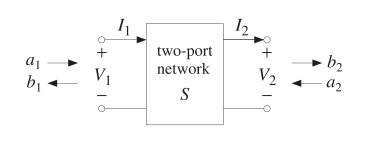
\includegraphics[width=8cm]{two_port.png}
\end{figure}

\begin{figure}[ht]
\label{Equivalent_Circuit}
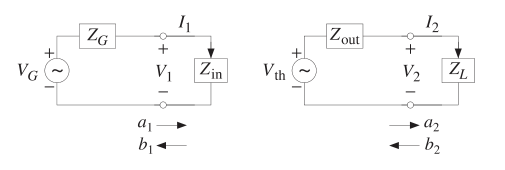
\includegraphics[width=8cm]{Equivalent_Circuit.png}
\end{figure}

\begin{align*}
\label{s-conversion-z}
Z_{11} &= Z_0\frac{(1+S_{11})(1-S_{22})+S_{12}S_{21}}{ (1-S_{11})(1-S_{22})-S_{12}S_{21}} \\
Z_{12} &= Z_0\frac{2S_{12}}{ (1-S_{11})(1-S_{22})-S_{12}S_{21}} \\
Z_{21} &= Z_0\frac{2S_{21}}{ (1-S_{11})(1-S_{22})-S_{12}S_{21}} \\
Z_{22} &= Z_0\frac{ (1-S_{11})(1+S_{22})+S_{12}S_{21}}{ (1-S_{11})(1-S_{22})-S_{12}S_{21}}
\end{align*}

We can convert the found S-Parameters to Z parameters and get the model of our Device Under Test (DUT) as shown in the resistor network above.

\section{Transmembrane Potential}
It is generally accepted that the cell membrane can be represented by a dielectric shell$(\epsilon_1,\sigma_1)$. The core can be described by $(\epsilon_2,\sigma_2)$. These live cells contain negative charges inside and attract the positive charges, mainly potassium and soidium ions on the outside.The dielectric response of live cells is fundamentally different then dead cells. The main difference between the two is the membrane potential in live cells. The effect of the membrane potential is an accumulation of mobile electric charge carriers at the membrane surfaces. When you introduce a time-oscillating electric field, these charges move on the surface of the membrane. Since the mobility of these surface charges is relatively small, this effect appears only at low frequencies, typically $<10kHz$. In this range the relative dieletric permittivity of live cell suspensions can be as high as $10^6$. This phenomenon is know as the $\alpha-$relaxation effect\cite{dielectric-response}. There is a sharp frequency above which the ions can no longer follow the electric field. Above this frequency, the polarizability of the cells drastically decreases and the $\alpha$-effect disappears.

\section{Materials}

\begin{figure}[h]
\label{test-fixture}
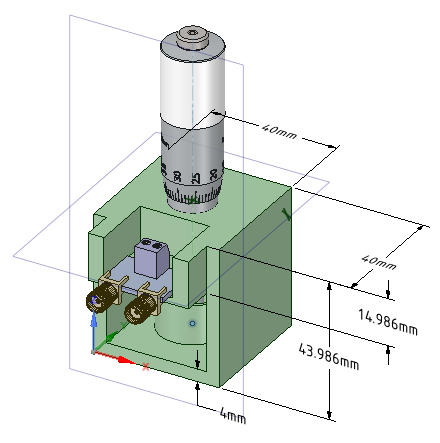
\includegraphics[width=8cm]{Combined_Test_Fixture.png}
\end{figure}

\subsection{Copper Plates}
Two copper plates $3/4 \: inch$ in diameter will be used. One plate will be fixed to the bottom of the beaker and the other is attached to a micrometer. To create the copper plates a hole puncher will be used.

\subsection{Copper Wire Leads}
Two wires will be attached to the copper plates. The wire attached to the fixed bottom plate will be attached to the center and run through the bottom of the test fixture to later be attached to a network analyzer.The second wire will be attached to top plate on one of the edges and run up the side of the beaker to be attached to a network analyzer. These two wires will provide the radio frequency signal and the probes to be attached to a network analyzer.

\subsection{3-D printed Beaker}
A 3-D printed beaker will be made to perfectly fit the test fixture. The beaker will be made of ABS plastic and is used to hold the cell suspension and two copper plates. It will be placed in the center of the Test fixture stand.

\subsection{Micrometer}
A micrometer will be used to adjust the height of one of the copper plates. The micrometer will be attached to the test fixture stand, and the drive of the micrometer will be attached to one of the copper plates. A micrometer cap will be 3-D printed in ABS plastic to perfectly fit the micrometer and later be adhered to the copper plate.

\subsection{Test Fixture Stand}
Provide a base for the beaker as well as an accurate and stable micrometer mount.This item will be 3D printed with ABS plastic.

\subsection{Cells}
SP 2/0 myelomas hypridoma cell line. These are nonadherent cells, and are essentially cancer cells from mice.\cite{mouse-myeloma-hybridoma-strain} They are rated at biosafety level 1. This level is suitable for work involving well-characterized agents not known to consistently cause disease in healthy adult humans, and of minimal potential hazard to laboratory peronnel and the environment. Reasearch with these agents may be performed on standard open laboratory benches without the use of special containment equipment and it is not necessary for Biosafety level 1 labs to be isolated from the general building.\cite{biosafety-levels}

\subsection{Hewlett-Packard 8735E Network Analyzer 30kHz - 6GHz}
Used with this network analyzer was the Agilent 11857D 7mm test port returns($50\Omega$). This network analyzer was used to gather our scattering parameters. This version features the 006 option which give it a 6 GHz upper frequency range.\\
Resolution: $1 Hz$ \\
Stability: typically $\pm7.5 ppm$ \\
Accuracy: $\pm10 ppm$\\
Resolution: $0.05 dB$

\begin{figure}[h]
\label{test-fixture}
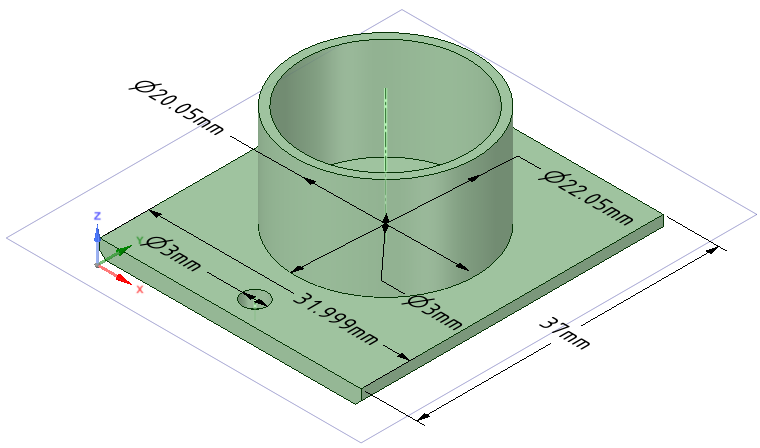
\includegraphics[width=8cm]{Beaker.png}
\end{figure}

\section{Methods}

\subsection{Cell Concentration}
The cell concentration will be measured using a hemocytometer. An example of the process of counting the cells can be seen in figure

\begin{figure}[h]
\label{hemocytometer}
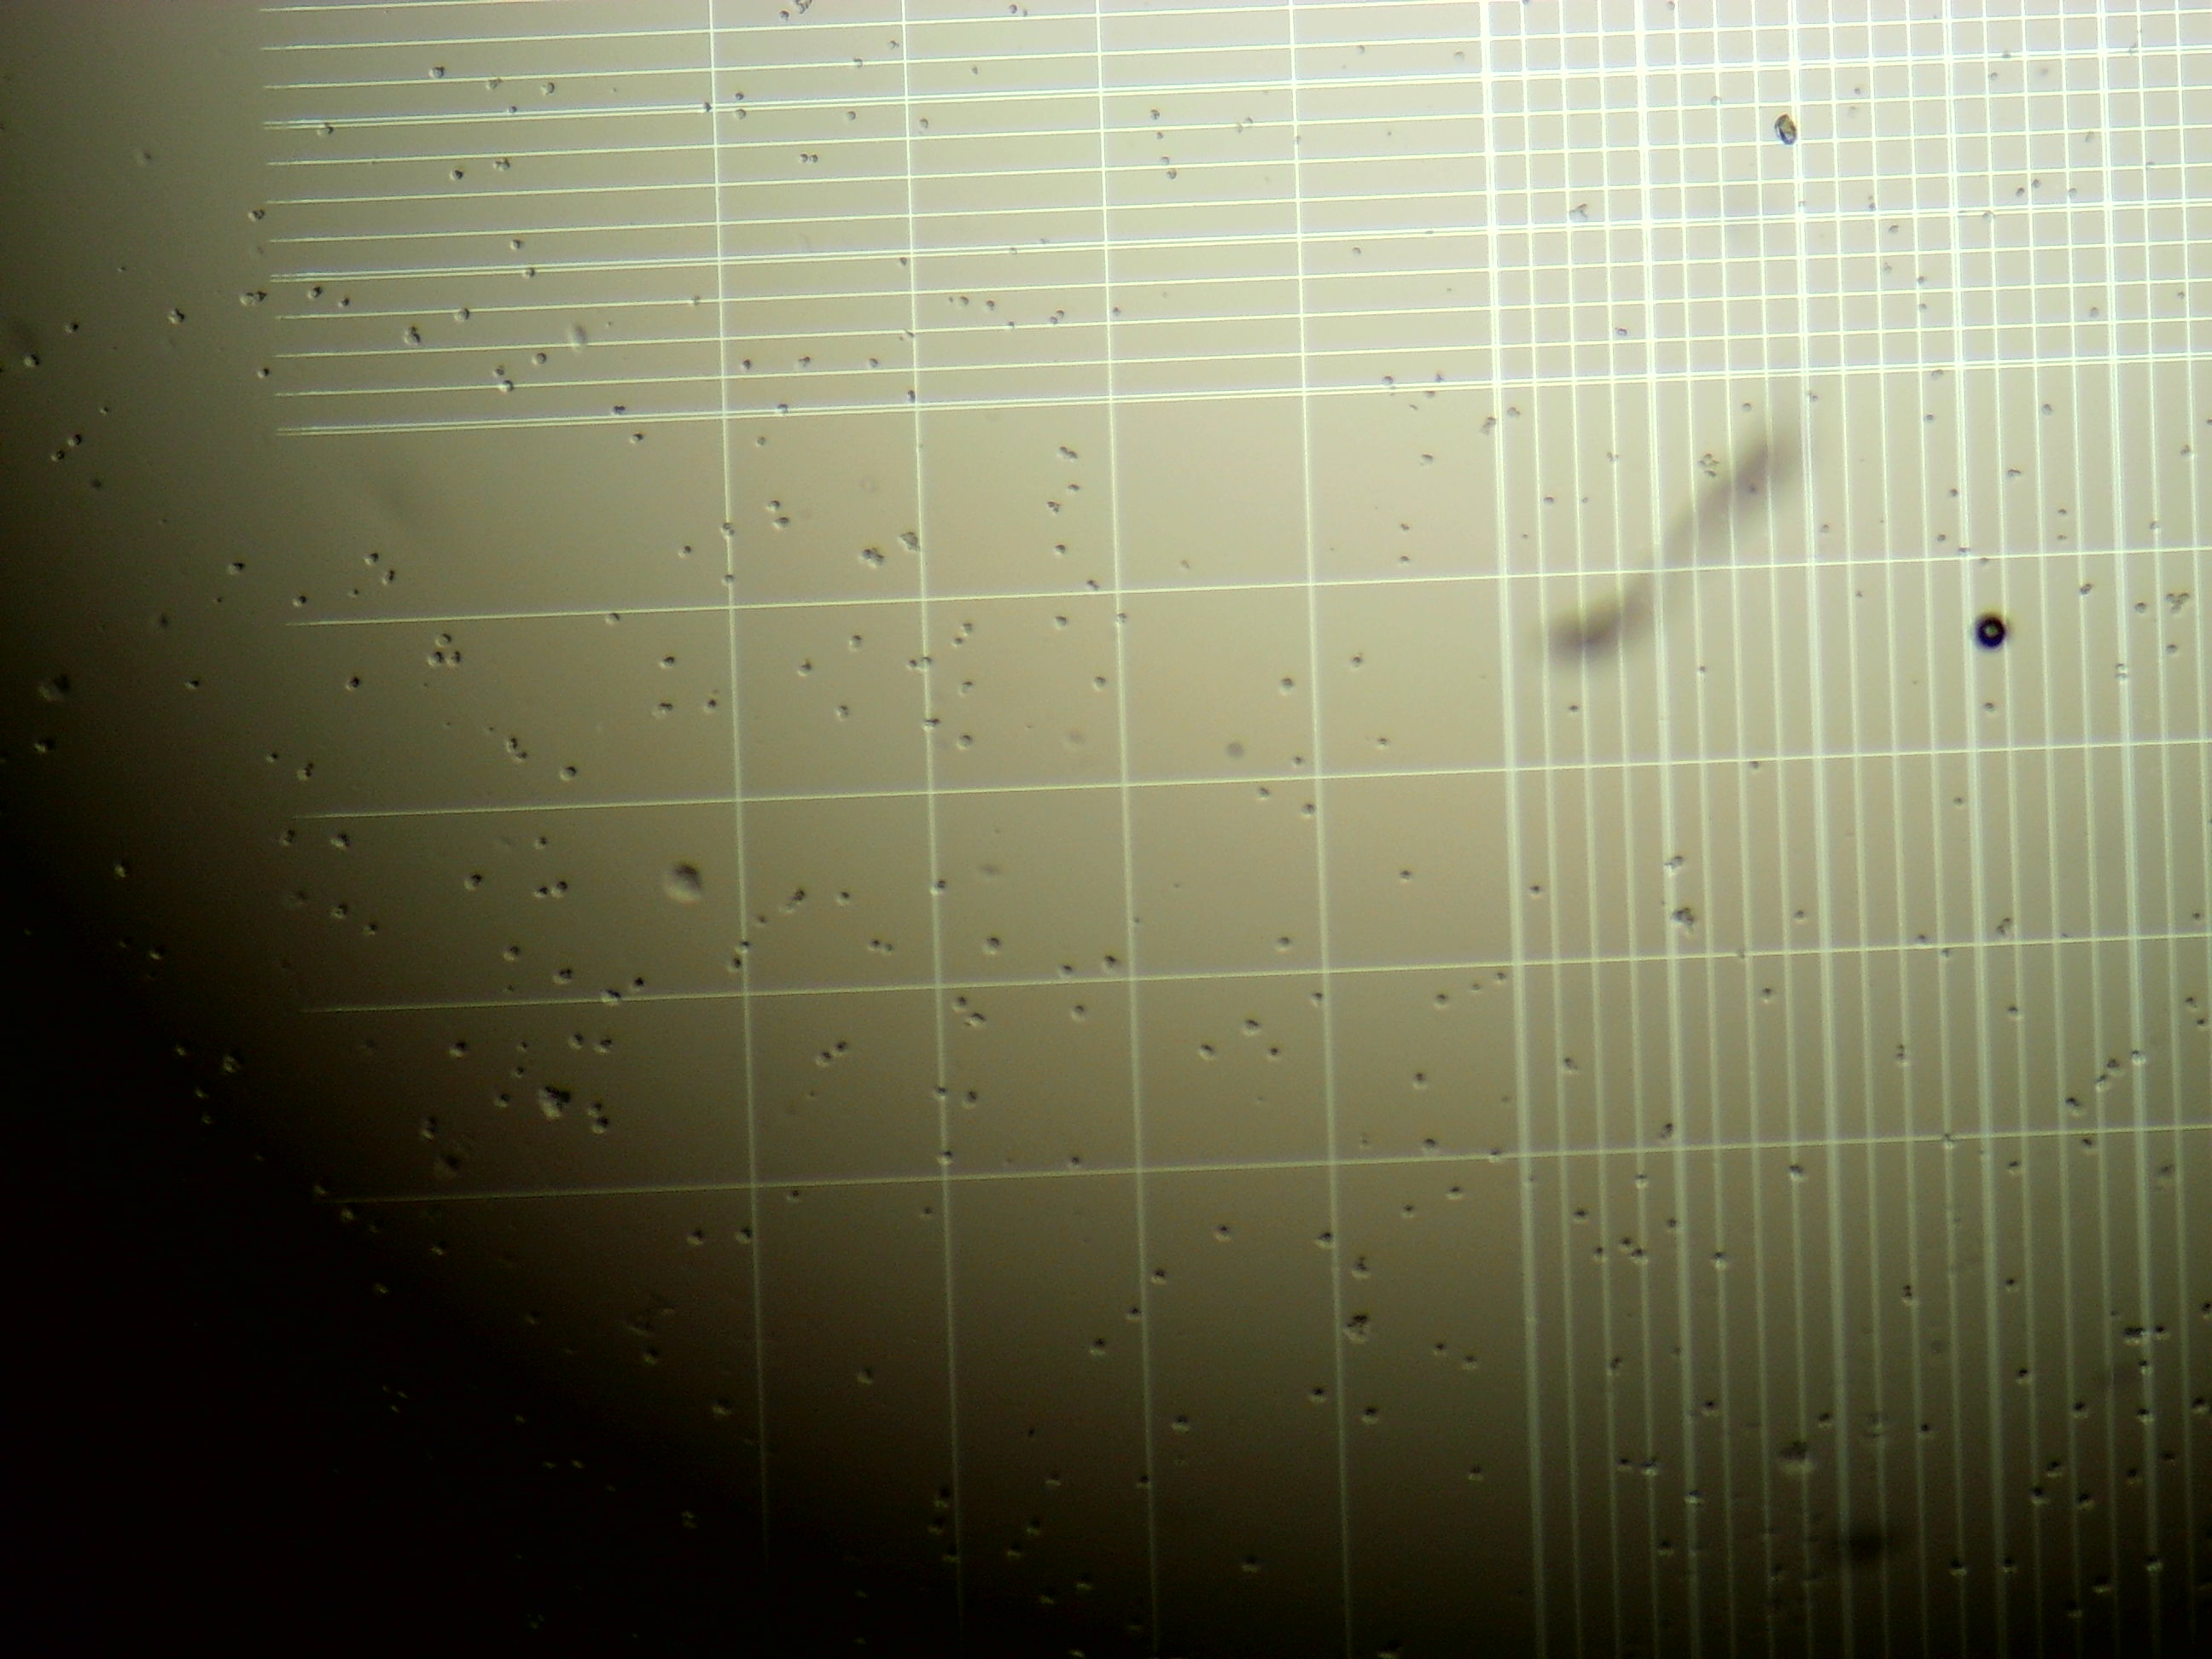
\includegraphics[width=9cm]{hemocytometer.jpg}
\end{figure}

\section{Procedure for splitting cells for regrowth and testing}
\subsection{Tools and Equipment}
\begin{itemize}
\item New cell culture flask
\item Centrifuge
\item 1ml centrifuge vials 
\item Pipette with 10ml graduated tips
\item Bleach
\item Phosphate buffer solution (PBS)
\item Cell food (10\% FBS PFS solution)
\item Vial rack for the centrifuge vials
\item 50ml sealable test tube
\end{itemize}

\subsection{Personal Safety Equipment}
For bio safety level 2, use of hood, gloves, and lab coat for person protection. With the hood shield down, protective eye ware was not needed. The hood should be turned on, and the shield lowered so only your hands can fit underneath it,  before any work with the cells is done. The cells are not to leave the bio safety level 2 lab room.

\subsection{Notes}
\begin{itemize}
\item The cell suspension will become more acidic over time, and thus, the more yellow or orange than dark pink (the color of the cell food).
\item The cells are being kept under conditions of 37 $\circ C$ and 4.9\% CO2 in the incubation chamber when not in use. 
\item The food is being stored in a standard refrigerator in a bio safety lab room.
\item The process does not need to leave the room to be completed.
\end{itemize}

\subsection{Procedure}

\textbf{Centrifuging:}
\begin{enumerate}
\item Remove the flask from the incubation unit and place it in the hood
\item Using the pipettes, put 1 ml of cell solution from the cell culture flask into each of the centrifuge vials until no more solution in the flask. 10 vials should be full.
\item Seal the vials, and evenly distributed them in a centrifuge which is then run at 1.7krpm for 5 min. Once complete, there will be a pellet of cells in the bottom of those vials. If there is an odd number of vials, do not use the odd one, place it aside on the rack for later disposal.
\item Split the vials into two equal groups. One group will be used to create the solution for testing and the other will be used to regrow the cell population.
\end{enumerate}

\textbf{For cell regrowth:}
\begin{enumerate}
\item Siphon off the solution in the vials and put it in the test tube. 
\item Using a new pipette, add 1ml of food to the vials. The tip of the pipette will not touch the cells.
\item Shake the vials to dissolve the pellet.
\item Using a pipette, add the solution of cells and cell food to a new cell culture flask. The flask should be labeled with the type of cells or strain, and what path number they are on.
\item The flask is then sealed, and placed horizontally back in the incubation chamber until this process needs to be repeated.
\end{enumerate}

\textbf{Preparing Cells for testing:}
\begin{enumerate}
\item Repeat step 1 from the Cell regrowth section
\item Using the pipette, add 1 ml of a buffer solution, phosphate saline buffer solution is added to the vials
\item Repeat step 3 of the Cell Regrowth section
\item Using the pipette, the solution can be added as needed to the test fixture. It can also be stored temporarily in test tube or a cell culture flask.
\end{enumerate}

\textbf{For unused centrifuge vials:}
\begin{enumerate}
\item Repeat step 1 from the Cell regrowth section
\item Using the pipette, add 1ml of bleach to the vials
\item Shake the vials to dissolve
\item Using a pipette, the bleach and cell solution is added to the mixture of old cells already in the disposable test tube. 
\end{enumerate}

\textbf{Clean up:} \\
If the disposable test tube has not had bleach added to it, several milliliters should be added to it. The liquid should turn light blue to clear, and now can safely be disposed. All surfaces in the hood and materials that are not disposable should be wiped down with 70\% ether solution. All equipment used that is disposable should disposed of in bio-safe bins which should be located near the hood. 

\section{Experiment Procedure}

\textbf{Initial Setup}
Set the test beaker to 10 mm spacing in between plates. The first plate is located where the micrometer reads 1 mm. Connect the Agilent 11857D 7mm test port returns($50\Omega$) to the network analyzer and the SMA connectors located on the test fixture. Both wires must be screwed into lead terminals. Before moving the top plate to the desired position, insert the fluid under test. Record all measurements to the floppy disc and copy the floppy disc to be further processed. 

\textbf{Measurements of S-Parameters:}
\begin{enumerate}
	\item Initially we will measure the S-Parameters of our device with air as a dielectric.
	\item Measure S-Parameters with PBS (Phosphate Buffered Saline).
	\item Measure S-Parameters with PBS Mouse Hybridoma solution.
\end{enumerate}

\textbf{Count Cell concentration}
Using the method as described earlier with the hemocytometer, count the cell concentration.

\section{Conclusion}
We hypothesised that using dielectric spectroscopy, on mouse hybridoma cells when exposed to a range of radio frequencies will cause a constant relative dielectric permittivity.Having this constant relative permittivity would lead to the conclusion that no potential exists at radio frequencies or that dielectric spectrosopy is not a viable solution to measure the trans-membrane potential at radio frequncies.A reason this may not be a viable solution is the fact the the radio-frequencies are passing through our dielectric as a short. If you look at the impedance for a capacitor $Z = \frac{1}{j2\pi f C}$ you will notice that as the frequency increases the impedance lowers. This means the electromagnetic waves will pass through the capacitor like a short, or in our case will pass through our cells. It is also known from prior research that an $\alpha$-relaxation effect occurs at frequencies lower than 10 kHz. Above this frequency the ions can no longer follow the electric field.

\section{Acknowledgement}
The authors would like to acknowledge Daniel Ewert and Jared Hansen for their leadership in this project. A special thanks to Dhamakeerthi Nawarathna for his help in the biology lab.

\begin{thebibliography}{9}

\bibitem{Dielectric Spectroscopy}
C.Prodan \textit{et al.},
"Low-frequency, low-field dielectric spectroscopy of living cell suspensions,"
\textit{Journal of Applied Physics}, 2004.

\bibitem{wave-propagation-water}
Shan Jiang and Stavros Georgakopoulos,
"Electromagnetic Wave Propagation into Fresh Water,"
\textit{Journal of Electromagnetic Analysis and Applications},2011,pp.261-266.

\bibitem{near-far-em}
Lou Frenzel,
What is the Difference Between EM Near Field and Far Field
\textit{Electronic Design}, 2012.

\bibitem{TMP-implications}
Brook T.Chernet and Michael Levin,
Transmembrane voltage potential is an essential cellular parameter for the detection and control of tumor development in a Xenopus mode,l\textit{Disease Models \& Mechanisms}2013,pp.595-607.

\bibitem{biosafety-levels}
Center for Disease Control and Prevention
\textit{Recognizing the Biosafety Levels}.
\url{www.cdc.gov/training/QuickLearns/biosafety/}

\bibitem{mouse-myeloma-hybridoma-strain}
ATCC
\textit{Mouse Hybridoma (Sp 2/0), IMM010.51.2 (PTA-2360)}.
American Type Culture Collection

\bibitem{Electromagnetic Waves and Antennas}
Sophocles J. Orfanidis,
Electromagnetic Waves and Antennas
\textit{Rutgers University},1999

\bibitem{dielectric-response}
Emil Prodan \textit{et al.},
"The Dielectric Response of Spherical Live Cells in Suspension: An Analytic Solution," \textit{Biophysical Journal}, 2008

\end{thebibliography}

\end{document}
>>>>>>> 52327035ade911616ac9466469c39f87a5ff8f86
